\documentclass[border=2pt]{standalone}
\usepackage{tikz}
\begin{document}
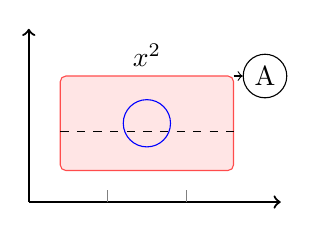
\begin{tikzpicture}
  % axes
  \draw[->, thick] (0,0) -- (3.2,0);
  \draw[->, thick] (0,0) -- (0,2.2);
  % panel with a rounded, filled rectangle
  \draw[red!70, fill=red!10, rounded corners=2pt]
    (0.4,0.4) rectangle (2.6,1.6);
  % dashed baseline inside the panel
  \draw[dashed] (0.4,0.9) -- (2.6,0.9);
  % circle and node
  \draw[blue] (1.5,1.0) circle (0.3);
  \node[draw, circle, inner sep=2pt] (A) at (3.0,1.6) {A};
  \draw[->] (2.6,1.6) -- (A.west);
  % tick marks
  \foreach \x in {1,2} {\draw[gray] (\x,0) -- (\x,0.15);}
  % label
  \node[above] at (1.5,1.6) {$x^2$};
\end{tikzpicture}
\end{document}
